
\section{Určenie náklonu zbrane}
Pre určenie náklonu zbrane v troch osách boli navrhnuté dve architektúry konvolučných neurónových sietí.
Každá z týchto sieti bola natrénovaná trikrát kvôli trom osám rotácie.
Nastavenia sieti boli opísane v návrhu.

Pre trénovanie v osi pitch bolo použitých 1036 obrázkov, na validáciu 222 a taktiež 222 pre testovanie presnosti siete.
V osi roll bolo na trénovanie použitých 3315 obrázkov, na validáciu 668 a 667 pre testovanie.
Nakoniec pre os yaw bolo použitých 3220 obrázkov na trénovanie a po 690 na validáciu a testovanie.
Všetky tieto obrázky prešli augmentáciou dát ako je opísane v \ref{subsec:augmentacia}.

\subsubsection{Pitch}
Sieť bola trénovaná v 50 epochách.
Priebeh trénovania obydvoch sieti pre os Pitch je vidieť na obrázku \ref{pic:pitchaxis}.
Kde pre presnosť týchto sietí je použitá metrika opísana v \ref{subsec:presnostmodelov}.
Hodnoty $angle\_error$ zobrazujú celkovú presnosť sieťe vzhľadom na priemernu odchylku uhla pre trénovacie dáta,
    $val\_angle\_error$ určuje túto odchylku pre validačné dáta.

\begin{figure}[H]
    \centering
    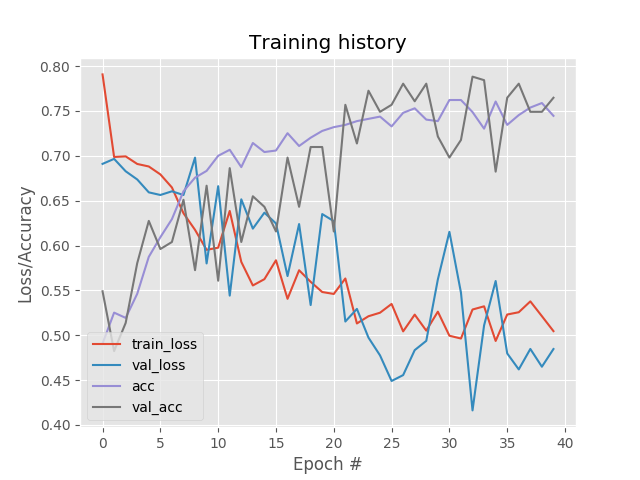
\includegraphics[width=0.49\textwidth]{alexnet-training_history}
	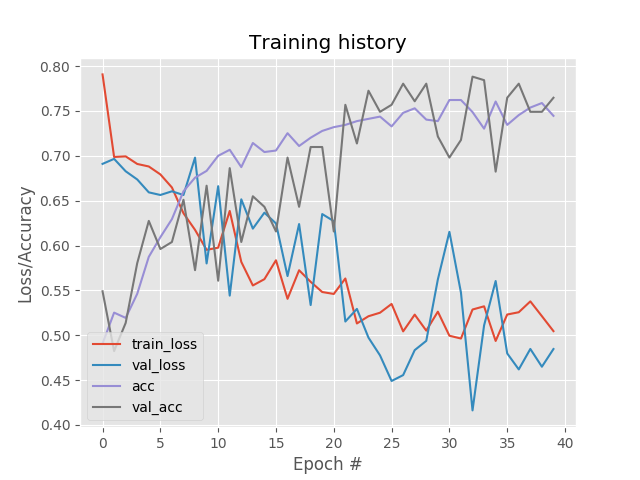
\includegraphics[width=0.49\textwidth]{alexnet-training_history} %vgglike-yaw5-training_history
	\caption{Priebeh trénovania sieti AlexNetLike(vľavo) a VGGLike(vpravo).}
	\label{pic:pitchaxis}
\end{figure}

Výsledna presnosť sieti je uvedená v tabuľkách \ref{tab:alexnetpitchresults} a \ref{tab:vgglikepitchresults} pre dve prahové hodnoty 5 a 10.

\begin{table}[H]
    \centering
    \begin{tabular}{|c|c|c|c|}
        \hline
        Prahová hodnota & V prahovej hodnota       & Mimo prahovej hodnoty    & Úspešnosť    \\ \hline
        5               & {\color[HTML]{009901} -} & {\color[HTML]{9A0000} -} & \textbf{-\%} \\ \hline
        10              & {\color[HTML]{009901} -} & {\color[HTML]{9A0000} -} & \textbf{-\%} \\ \hline
    \end{tabular}
    \caption{Výsledky natrénovanej siete AlexNetLike pre os Pitch.}
    \label{tab:alexnetpitchresults}
\end{table}
\begin{table}[H]
    \centering
    \begin{tabular}{|c|c|c|c|}
        \hline
        Prahová hodnota & V prahovej hodnota       & Mimo prahovej hodnoty    & Úspešnosť    \\ \hline
        5               & {\color[HTML]{009901} -} & {\color[HTML]{9A0000} -} & \textbf{-\%} \\ \hline
        10              & {\color[HTML]{009901} -} & {\color[HTML]{9A0000} -} & \textbf{-\%} \\ \hline
    \end{tabular}
    \caption{Výsledky natrénovanej siete VGGLike pre os Pitch.}
    \label{tab:vgglikepitchresults}
\end{table}


\subsubsection{Roll}
Trénovanie prebiehalo rovnako ako v Pitch osi.

\begin{figure}[H]
    \centering
    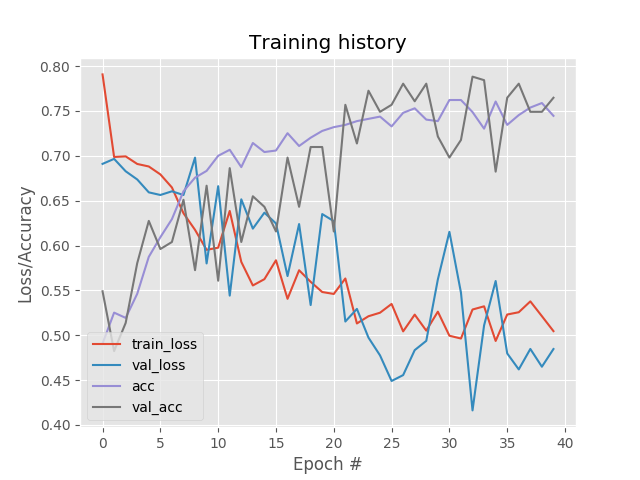
\includegraphics[width=0.49\textwidth]{alexnet-training_history} %vgglike-roll-training_history
	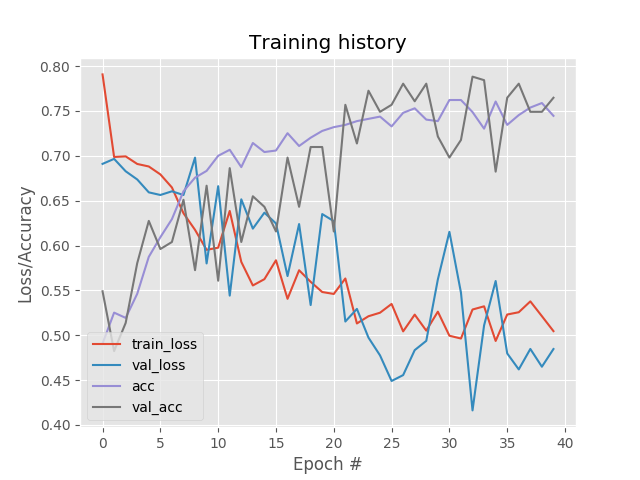
\includegraphics[width=0.49\textwidth]{alexnet-training_history} %vgglike-roll-training_history
	\caption{Priebeh trénovania sieti AlexNetLike(vľavo) a VGGLike(vpravo).}
	\label{pic:rollaxis}
\end{figure}

\begin{table}[H]
    \centering
    \begin{tabular}{|c|c|c|c|}
        \hline
        Prahová hodnota & V prahovej hodnota       & Mimo prahovej hodnoty    & Úspešnosť    \\ \hline
        5               & {\color[HTML]{009901} -} & {\color[HTML]{9A0000} -} & \textbf{-\%} \\ \hline
        10              & {\color[HTML]{009901} -} & {\color[HTML]{9A0000} -} & \textbf{-\%} \\ \hline
    \end{tabular}
    \caption{Výsledky natrénovanej siete AlexNetLike pre os Roll.}
    \label{tab:alexnetrollresults}
\end{table}
\begin{table}[H]
    \centering
    \begin{tabular}{|c|c|c|c|}
        \hline
        Prahová hodnota & V prahovej hodnota       & Mimo prahovej hodnoty    & Úspešnosť    \\ \hline
        5               & {\color[HTML]{009901} -} & {\color[HTML]{9A0000} -} & \textbf{-\%} \\ \hline
        10              & {\color[HTML]{009901} -} & {\color[HTML]{9A0000} -} & \textbf{-\%} \\ \hline
    \end{tabular}
    \caption{Výsledky natrénovanej siete VGGLike pre os Roll.}
    \label{tab:vgglikerollresults}
\end{table}


\subsubsection{Yaw}
Priebeh trénovania a výsledky pre os Yaw.

\begin{figure}[H]
    \centering
    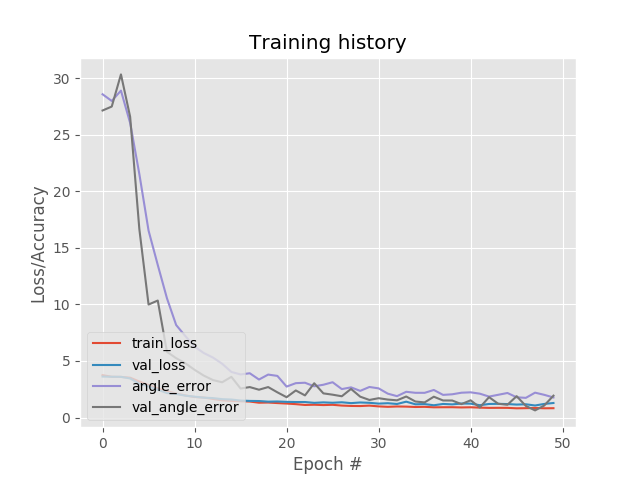
\includegraphics[width=0.49\textwidth]{alexnet-yaw5-training_history}
	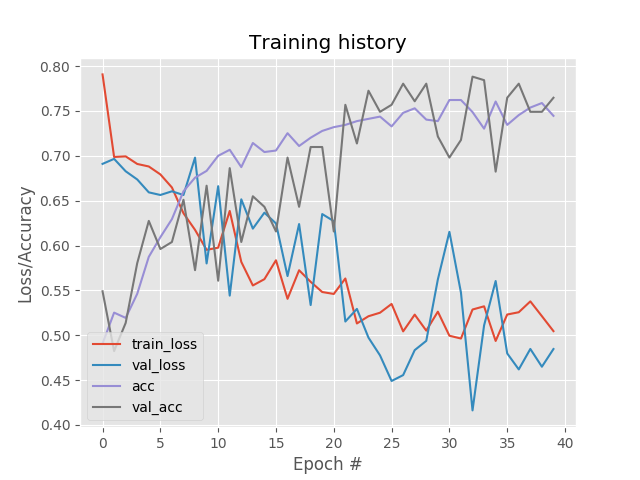
\includegraphics[width=0.49\textwidth]{alexnet-training_history} %vgglike-yaw-training_history
	\caption{Priebeh trénovania sieti AlexNetLike(vľavo) a VGGLike(vpravo).}
	\label{pic:yawaxis}
\end{figure}

\begin{table}[H]
    \centering
    \begin{tabular}{|c|c|c|c|}
        \hline
        Prahová hodnota & V prahovej hodnota       & Mimo prahovej hodnoty    & Úspešnosť    \\ \hline
        5               & {\color[HTML]{009901} 342} & {\color[HTML]{9A0000} 346} & \textbf{49.71\%} \\ \hline
        10              & {\color[HTML]{009901} 376} & {\color[HTML]{9A0000} 312} & \textbf{54.65\%} \\ \hline
    \end{tabular}
    \caption{Výsledky natrénovanej siete AlexNetLike pre os Yaw.}
    \label{tab:alexnetyawresults}
\end{table}
\begin{table}[H]
    \centering
    \begin{tabular}{|c|c|c|c|}
        \hline
        Prahová hodnota & V prahovej hodnota       & Mimo prahovej hodnoty    & Úspešnosť    \\ \hline
        5               & {\color[HTML]{009901} -} & {\color[HTML]{9A0000} -} & \textbf{-\%} \\ \hline
        10              & {\color[HTML]{009901} -} & {\color[HTML]{9A0000} -} & \textbf{-\%} \\ \hline
    \end{tabular}
    \caption{Výsledky natrénovanej siete VGGLike pre os Yaw.}
    \label{tab:vgglikeyawresults}
\end{table}
